\section{Baryons}
A Baryon is a subatomic particle. It is composite and contains three quarks.
The Baryons form together with the mesons the class of the hadrons. Mesons are 
composed of two quarks, one quark and one antiquark.\\
Protons and neutrons which are the components of our normal matter are baryons. 
These are the lightest baryons. The proton is made of two up quark and one down 
quark. The neutron contains two down quark and one up quark.\\
All observed events so far feature that the number of baryons in a reaction is 
observed. To use this in calculations every quark get the baryon number \(B = 1/3\) and 
every anti-quark \(B = -1/3\). In a decay from a baryon (\(\sum B = 1\)) the final 
products has to be a baryon (\(\sum B = 1\)) or two baryons (\(\sum B = 2\)) 
and an anti-baryon (\(\sum B = -1\)) and so on. 

\subsection{\(\Lambda_c^+\) Baryon}
The \(\Lambda_c^+\) has a mass of \(2286.46 \pm 0.14 \text{MeV}^
{\text{\cite{lambda-pdg}}}\) and a mean life time of \(\left( 2.00 \pm 0.06\right)
\cdot 10^{-13} \text{s}^{\text{\cite{lambda-pdg}}}\). It is one of the lightest charmed 
baryons and is made of one up, down and charm quark. His charge is +1 of the 
electron charge\(^{\text{\cite{lambda-pdg}}}\).

\section{Decays}
Decays are processes with one particale in the initial state and n particles 
in the final state for n= 2,3,{\ldots}. The decayed particle mustn't be in the final 
state. This makes the difference to rediation processes. The decay process can 
always be transformed in the rest mass frame of the Decayer and so the 
summation over the energy of all particles in the final state has to be the 
rest energy of the decaying particle.\\
A decay process or more general a transision process is characterized through 
Fermi's golden rule{\eqref{eq:fermi}}.
\begin{equation}
  \Gamma_{fi} = 2 \pi |T_{fi}|^2 \rho\left(E_i\right) \label{eq:fermi}
\end{equation}
In equation{\eqref{eq:fermi}} \(T_{fi}\) is the transition matrix element and 
\(\rho\left(E_i\right)\) is the density of states. The result is the transition 
rate \(\Gamma_{fi}\).In natural units the unit of the transition rate is \(\text{GeV}^{-1}\).\\
For decay process the only one intial is possible, the decayer and f is often 
labeled as i in literature. And so Fermi's golden rule becomes to equation
{\eqref{eg:width}}.
\begin{equation}
  \Gamma_i = 2 \pi |T_i|^2 \rho\left(E\right) \label{eq:width}
\end{equation}
The \(\Gamma_i\) is called partial decay width. And is characteristic value 
for a decay process. The sum over all partial decay widths is called 
total decay width{\eqref{eq:total}}.
\begin{equation}
  \Gamma = \sum_i \Gamma_i \label{eq:total}
\end{equation}
The total width{\eqref{eq:total}} is an criterion for the lifetime of the 
decaying particle. The lifetime{\eqref{eg:lifetime}} of the particle in natural units is the 
inverse of \(\Gamma\).
\begin{equation}
  \tau = \frac{1}{\Gamma} \label{eq:lifetime}
\end{equation}
The branching ratio{\eqref{eq:br}} is the probability to decay in a specific final 
state. It can be calculated with the partial and total decay width.
\begin{equation}
  BR( i \rightarrow f) = \frac{\Gamma_f}{\Gamma} \label{eq:br}
\end{equation}
The formula {\eqref{eq:br}} use the same indices like equation{\eqref{eq:fermi}}.

\section{Weak Decay}
A weak decay is the transition of a particle through the weak interaction. An 
elementary particle that is possibly part of an composite can in this 
way decay to a W\(^\pm\)-Boson and an correspondending part. But the W-Boson only 
couple to lef-handed fundamental partciles and right-handed fundamental 
anti-particles. The spinor for the weak interaction than looks like 
{\eqref{eq:spinor}}. There the upper have isospin -1/2 and the lower isospin 
+1/2.
\begin{equation}
  \Spvek{\nu_e; e}_L,\Spvek{\nu_\mu; \mu}_L, \Spvek{d; u}_L, \Spvek{s; c}_L, 
  \text{ etc.} \label{eq:spinor}
\end{equation}
In {\eqref{eq:spinor}} only the important particles are shown.\\
The value for a W\(^\pm\) propagator is \(\propto \frac(1){q^2 - m_W^2}\). But 
in most process the transfered momentum is much lower compared to the Mass of 
the W\(^\pm\) boson because it is the mass 
difference of the initial particle and the final particle that are connected 
through the W\(^\pm\) vertex. This leads to an estimation there the propagator 
becomes to \(\propto \frac(1){m_W^2} \propto G_F\). \(G_F\) is the Fermi constant 
for the weak interaction and the process looks like a one to three vertex because 
W\(^\pm\) boson is not stable and decays in other particles.\\
The measurement of leptons are mostly very accurate in a detector and 
the calculation of the transisition matrix element becomes easier for leptonic 
decays only this decays are considered. For the \(\Lambda_c^+\) exists the 
following Feynman diagram{\eqref{fey:lambda}}. The \(\Lambda_c^+\) can decay 
in a neutron or a Lambda as baryon and a positron or anit-muon as lepton plus 
the correspondending neutrino to observe the lepton number.
\begin{figure}[h]
  \centering
  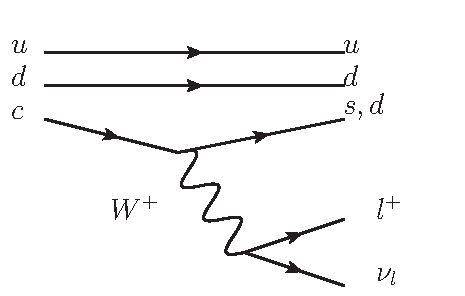
\includegraphics[page=1, width=0.5\textwidth]{semileptonic_lambdac+}
  \caption{Semileptonic decay modes of the \(\Lambda_c^+\) into a neutron (udd)
  or a \(\Lambda\) (uds), an positron or an anti-muon and the correspondending 
  neutrino (own graphic)}\label{fey:lambda}
\end{figure}

\section{V-A current}
The value of a Vertex where two pertinent leptons transforms into a  
W\(^\pm\) boson is \(-i \frac{g}{2\sqrt{2}} \gamma^\mu\left(1-\gamma^5\right)\).
If the sum is splitted, the the term without \(\gamma^5\) is called vector and 
the part with the \(\gamma^5\) axial-vector through the geometrical effect of 
the \(\gamma\)-matrix. The transition from quarks needs an additional factor 
\(V_{if}\). i is the quark and in the initial state and f the quark in the 
final state. The factor comes from the CKM-matrix\(^{\text{\cite{ckm}}}\). The 
matrix from {\cite{ckm}} is shown in {\eqref{eq:ckm}}.
\begin{equation}
  V_{CKM} =
  \begin{bmatrix}
    0.97434^{+0.00011}_{-0.00012} &  0.22506 \pm 0.00050 & 0.00357 \pm 0.00015 \\
    0.22492 \pm 0.00050 & 0.97351 \pm 0.00013 & 0.0411 \pm 0.0013 \\
    0.00875^{+0.00032}_{-0.00033} & 0.0403 \pm 0.0013 & 0.99915 \pm 0.00005
  \end{bmatrix} \label{eq:ckm}
\end{equation}
With the general Feynman rules for vertices and propagators the transition matrix 
element becomes to {\eqref{eq:trans}} like in {\cite[Eq. 1]{Frank}}.
\begin{equation}
  T = \frac{G_F}{\sqrt{2}} V_{Qq} \bar{u_l}\gamma^\mu\left(1 - \gamma^5\right) 
  u_{\nu_l} \langle B(p', s') | J_\mu | \Lambda_c(p, s) \rangle \label{eq:trans}
\end{equation}
The B in {\eqref{eq:trans}} stands for the neutron or \(\Lambda\). The current 
\(J_\mu\) can be splitted in a vector-axial and an axial part \(J_\mu = V_\mu - 
A_\mu \) like in {\eqref{eq:v-a}}.
\begin{align}
  \langle B(p', s') | V_\mu | \Lambda_c(p, s) \rangle & = \bar{u}(p', s') 
  \left( F_1(q^2) \gamma_\mu + F_2(q^2)\frac{p_\mu}{m_{\Lambda_c}} + 
  F_3(q^2)\frac{p'_\mu}{m_B} \right) u(p, s) \nonumber \\
  \langle B(p', s') | A_\mu | \Lambda_c(p, s) \rangle & = \bar{u}(p', s') 
  \left( G_1(q^2) \gamma_\mu + G_2(q^2)\frac{p_\mu}{m_{\Lambda_c}} + 
  G_3(q^2)\frac{p'_\mu}{m_B} \right) \gamma^5 u(p, s) \label{eq:v-a}
\end{align}
The \(F_i\) and \(G_i\) are form factors for the transition. They are specific 
for the initial and final baryons and describe the different behavior of the 
quarks in a bound state in contrast to the free decay. The functional behavior 
of these form factors is related to \(q^2 = (p - p')^2\).

\section{Monte-Carlo basics}
The \texttt{Sherpa} software use Monte-Carlo methods to calcullate the 
dynamics of the process for the phase space integration of the partial width. 
To understand this method Fermi's golden rule{\eqref{eq:fermi}} has to be written 
as an integral. This integral can be ontained from the density of states. 
A formula like \cite[Eq. 2.38]{diploma} is the result of this equation. The 
differential dacay rate is an important part because with Monte-Carlo the 
integral can be performed. For this a point in the phase space is diced. The 
differential decay rate \(d\Gamma\) is calculated. If the Ratio between the 
differential decay rate and the maximum decay rate is bigger as a random 
number between zero and one the event is accepted. This points will be 
collected and form the integral and so the decay rate at the end.

